\fancychapter{Existing Trajectory optimization Methods for Motion Planning}%
\cleardoublepage%
% The following line allows to ref this chapter
\label{chap:theory}
%\todo[color=green!40, author=Thomas, fancyline]{choose best title for chapter}{}

\par In this chapter, Direct Methods for trajectory optimization will be reviewed. These methods are generic, i.e., they can be applied to a wide range of dynamic systems. Here, these methods are applied to the control of a vehicle in both one and two dimensions. A good understanding of motion planning for single vehicles will be necessary before extending to multiple vehicles.

\section{The Optimization Problem}
\label{sec:optimprob_intro}

\par Motion planning for a single vehicle can be cast in the form of an optimal control problem of the form (see \cite{diehl2006fast})

\begin{equation}
    \begin{aligned}
    & \underset{x(.),u(.)}{\text{minimise}} && J = \int_0^T L(x(t),u(t))dt + \Psi (x(T)) \ dt\\
    & \text{subject to}  && x(0) = x_0, \\
        & && \dot{x} = f(x(t), u(t)), &&& t \in [0,T] \\ % &&&& \text{(fixed initial value)} \\
        & && h(x(t),u(t)) \geq 0, &&&  t \in [0,T] \\ % &&&& \text{(ODE Model)}\\
        & && r(x(T)) = 0 % &&&& \text{(terminal constraints)} &&&&&
    \end{aligned}
    \label{eq:general_cost}
\end{equation}
where $x(t)$ is defined as $x:[0,T]\rightarrow \mathbb{R}^{n_x}$, $u(t)$ is defined as $u:[0,T]\rightarrow \mathbb{R}^{n_u}$, $f(x,t)$ is the system of equations for the dynamics, defined as $f:\mathbb{R}^{n_x}\times \mathbb{R}^{n_u}\rightarrow \mathbb{R}^{n_x}$, $x_0$ is the initial state, $h(x(t)$, $u(t))$ represents the path constraints, $r(x(T))=0$ the terminal constraints, $L(x(t),u(t))$ is the running cost, defined as $L:\mathbb{R}^{n_x}\times \mathbb{R}^{n_u}\rightarrow \mathbb{R}$, $\Psi(x(t))$ is the terminal cost defined as $\Psi:\mathbb{R}^{n_x} \rightarrow \mathbb{R}$ and finally $T$ is known as the time ”horizon”, i. e., no matter what motion planning algorithm is used, the produced control law will only be valid within time $t\in[0;T]$.

\par An example of a path constraint is to keep the minimum distance to a known obstacle bounded below by a desired safety distance. If $x$ encodes the position then $h(x)$ could be
\begin{equation}
    \label{eq:example_constr}
    h(x(t)) = \underset{t\in[0,T]}{\text{min}}\lVert x - p_0 \rVert - d_{\text{min}}
\end{equation}
where $p_0$ is the location of an obstacle's centre of mass and $d_{\text{min}}$ is the minimum accepted distance to that centre.

\par All of the available Direct Methods used in this Thesis have as an objective the formulation of a control law that optimises some form of the above cost function. These methods will be demonstrated with the control of a double integrator in 1-D and 2-D. A double integrator is a linear system where the second derivative of the position variable $y$, is the acceleration $a$, that is,
\begin{equation}
    \ddot{y} = a
    \label{eq:basic_double_int}
\end{equation}
\par A general linear system is represented, in state-space form, by
\begin{equation}
    \dot{x} = Ax + Bu
    \label{eq:general_state_space}
\end{equation}
where $x = [x_1,\dots,x_{n_x}]^T$ is the state of the system and $u = [u_1,\dots,u_{n_u}]^T$ is the input. For the double integrator, the states and inputs are given by
\begin{equation}
\begin{cases}
    x_1 = y \\ x_2 = v \\ u = a
\end{cases}
\end{equation}
where $x_1$ and $x_2$ represent position and velocity, respectively, and $u$ is the acceleration. The system's dynamics then become
\begin{equation}
    \label{eq:dynamics_double_int}
    \begin{cases}
        \dot{x}_1 = x_2 \\
        \dot{x}_2 = u
    \end{cases}
\end{equation}
or
\begin{equation}
    \begin{bmatrix}
    \dot{x}_1 \\ \dot{x}_2
    \end{bmatrix} = 
    \begin{bmatrix} 0 & 1 \\ 0 & 0 \end{bmatrix} 
    \begin{bmatrix} x_1 \\ x_2 \end{bmatrix} + 
    \begin{bmatrix} 0 \\ 1 \end{bmatrix} u
    \label{eq:state_space_double_int}
\end{equation}
in matrix form, which means matrices $A$ and $B$ of equation \ref{eq:general_state_space} are given by
\begin{equation}
    A = \begin{bmatrix} 0 & 1 \\ 0 & 0 \end{bmatrix}, \qquad B = \begin{bmatrix} 0 \\ 1 \end{bmatrix}
    \label{eq:A_and_B}
\end{equation}.

\par The cost function \ref{eq:general_cost} will be simplified to
\begin{equation}
    J = \int_0^\infty x_1^2 + x_2^2 + \rho u^2\  dt
    \label{eq:my_cost}
\end{equation}
where $\rho$ is a scalar that penalizes "energy" consumption.
\par This dynamic system is diferentially flat (see section \ref{sec:differentiallyflatsystems}) with $x_1$ as the flat output, because it is possible to express $x_2$ as a derivative of $x_1$ and $u$ as a double derivative of $x_1$.
\par Although this 1-D model is very simple, it can provide insight into real life applications. One obvious example is a train that follows a track. It cannot leave the track and so, environmental constraints, such as obstacles, cannot be fixed in time if they are between the train's initial and target position. A non-fixed constraint could be another train that is joining the same track, therefore, the first train cannot be at certain points at certain times.
\par The optimization problem \eqref{eq:general_cost}, is infinite dimensional because the solution will be a function of time, which has an infinite number of points. The following Direct Methods will replace the infinite number of points of the function by approximated functions which are parameterized by a finite number of variables.
\par Before presenting the Direct Methods, results of the application of the \acl{LQR} are presented. This is important as the results serve as baselines to compare with the Direct Methods. The \ac{LQR} is a feedback law which guarantees minimal cost for certain kinds of cost functionals.

\section{Linear Quadratic Regulator}
\label{sec:linearquadraticregulator}

\par A \acl{LQR} is a technique applicable to linear dynamic systems of the form
\begin{equation}
    \label{eq:dynamic_system}
    \dot{x} = A x + B
\end{equation}
using the same definitions as in section \ref{sec:optimprob_intro}.

\par The Linear Quadratic Regulator algorithm yields, under certain conditions, an appropriate state-feedback LQR controller that minimises a cost function of the form
\begin{equation}
    \label{eq:quadratic_cost}
    J = \int_0^\infty x^T Q x + u^T R u + 2x^T N u dt
\end{equation}

\par The control law is of the form
\begin{equation}
    \label{eq:feedback}
    u = -Kx
\end{equation}
where $K$ is given by
\begin{equation}
    \label{eq:k_expression}
    K = R^{-1} (B^T P(t) + N^T)
\end{equation}
where $P(t)$ is the solution of the differential Riccati equation \cite{riccati1724animadversiones}
\begin{equation}
    \label{eq:p_diff_expression}
    A^T P(t) + P(t) A - (P(t) B + N) R^{-1} (B^T P(t) + N^T) + Q = - \overline{P}(t)
\end{equation}
with appropriate boundary conditions.

\par For the situation where the time horizon $T$ is $\infty$, $P(t)$ will tend to a constant solution, $P$, and, as a result, $P$ is found by solving the continuous time algebraic Riccati equation 
\begin{equation}
    \label{eq:p_expression}
    A^T P + PA - (PB + N) R^{-1} (B^T P + N^T) + Q = 0
\end{equation}

%\par Note that the cost in this equation is for an infinite time horizon and for continuous-time linear systems given by \ref{eq:dynamic_system}. The feedback control law.

\par The solution provided by this algorithm will be optimal and unique if the following conditions are fulfilled:
\begin{itemize}
    \item $(A,B)$ is controllable;
    \item for a system output $y = C x$, with $Q=C^T C$, the pair $(A,C)$ is observable;
    \item $R>0$ and $Q>0$.
\end{itemize}

\par Control via LQR is in closed-loop form, which has the advantage of being robust against parameter uncertainty and reducing the effect of external disturbances. 
\par In order to visualise the resulting controlled double integrator evolves over time, the feedback law \eqref{eq:feedback} is fed into the system \eqref{eq:dynamic_system}, non zero initial conditions are provided, and the resulting \ac{IVP} is solved. In other words, the objective is to find the soltion to 
\begin{equation}
    \begin{aligned}
    & \dot{x} = (A-BK)x \\
    & \text{subject to} \quad x(0) = x_0
    \end{aligned}
    \label{eq:controlledlinearsystem}
\end{equation}
where $x_0$ is the initial conditions.

%\par The regulator parameters can only be obtained for a more specific subset of the cost functions of equation \ref{eq:general_cost}. These will be given in the form of equation \ref{eq:quadratic_cost}. Where Q and R are matrices.

%\par \texttt{Matlab} implements the solution of the quadratic regulator in the functions \texttt{lqr} (for continuous systems) and \texttt{dqlr} (for digital systems). % These functions calculate the solution to the Riccati equation.

\par Here an example of control of the double integrator is presented in the context of linear quadratic regulator theory. Here, the initial conditions, which will be the same for all the subsequent 1-dimensional examples throughout this chapter, are  given by
\begin{equation}
    \label{eq:initial_conds}
    x_0 = \begin{bmatrix} x_{1_0} \\ x_{2_0} \end{bmatrix} = \begin{bmatrix} 3 \\ 1 \end{bmatrix}
\end{equation}

\par Figure \ref{fig:solution_lqr} shows the of an \ac{LQR} controlled double integrator. The regulator used for this example was obtained with $Q = I$ and $R = \rho = 0.1$ as weights to obtain $K$ in equation \ref{eq:k_expression} so that the resulting cost matches \ref{eq:my_cost}.



%\begin{equation}
%    x = \begin{bmatrix}x_1 \\ x_2\end{bmatrix}, \qquad Q = \begin{bmatrix} 1 & 0 \\ 0 & 1 \end{bmatrix}, \qquad R = \rho, \qquad N = 0
%\end{equation}

\begin{figure}[h!]
\centering
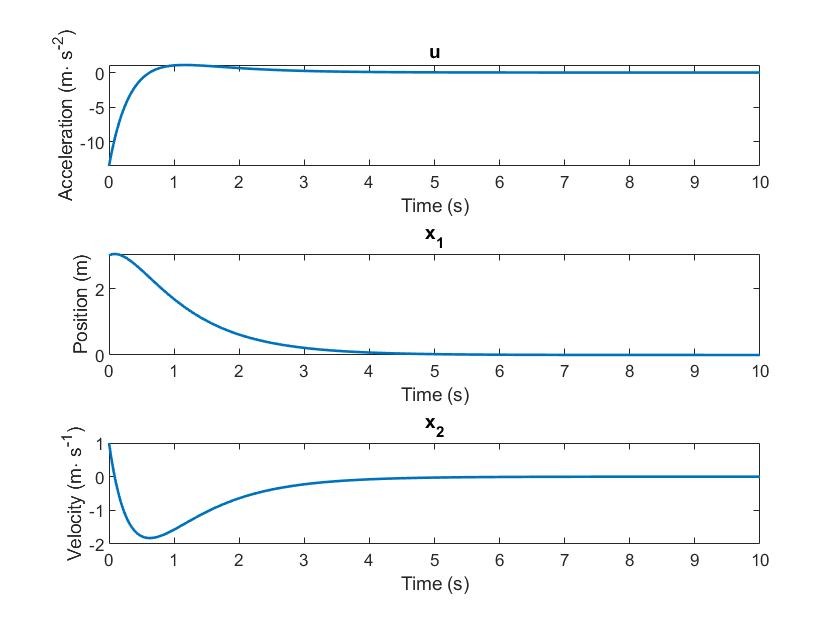
\includegraphics[width=0.8\textwidth]{Images/solution_lqr.jpg}
\caption{\acs{LQR}-Controlled Double Integrator Solution}
\label{fig:solution_lqr}
\end{figure}

\par It can be seen that all variables tend asymptotically to zero. It should be noted that after around 6 seconds the system can already be considered stationary.



\section{Single Shooting}
\label{sec:singleshooting}

\par Single Shooting is a direct method for motion planning. It consists of parameterising, for a given system, the control input signal $u(t)$ as a piece-wise constant function of time, as defined by 
\begin{equation}
    \label{eq:single_shooting}
    u(t) = q_i, \qquad t\in [t_i,t_{i+1}]
\end{equation}
where $q_i$ has the dimensions of the input, and the intervals $[t_i,t_{i+1}]$ denote the time-intervals between instants indexed by indices $i$ and $i+1$.

\par The following step consists of solving the following \ac{ODE}:
\begin{equation}
    \label{eq:ode_zoh}
    \begin{aligned}
        & x(0) = x_0, \\
        & \dot{x}(t) = f(x(t),u(t;q)), && t\in[0,T].
    \end{aligned}
\end{equation}
to obtain the time evolution of $x$.

\par With the obtained trajectories, the optimization problem (\ref{eq:general_cost}) can be extended and expressed as a function of the parameters $q=(q_0,q_1,\dots,q_{N-1})$ as optimization variables. The new optimization problem is written in the form  
\begin{equation}
    \begin{aligned}
    & \underset{q}{\text{minimise}} && \int_0^T L(x(t;q),u(t;q))dt + \Psi (x(T;q)) \ dt \\
    & \text{subject to}  && x(0) = x_0, \\
        & && \dot{x} = f(x(t), u(t)), &&& t \in [0,T]  \\
        & && h(x(t),u(t)) \geq 0, &&&  t \in [0,T]  \\
        & && r(x(T)) = 0
    \end{aligned}
    \label{eq:cost_zoh}
\end{equation}

\par This method can produce good results when a sufficiently low step duration is used. However, an important concern when compared to other methods is the computation time. Convergence for a good solution takes a long time because the number of parameters that are used is relatively large. With an increasing number of search parameters comes a increasingly bigger complexity and, because the cost can only be calculated for the completed trajectory, calculating the gradients with respect to each parameter can be very difficult.

\par Trajectory planning for the double integrator with single shooting will be unconstrained. This is because the solution produced by the optimization problem will shape $u$, which will have no influence on the problem's initial conditions. 
\par The solution for this unconstrained problem can be found using the Matlab function \texttt{fminsearch}.
\par During the optimization process, the variables $x_1$ and $x_2$ will be necessary for calculation of the cost. The integral \ref{eq:my_cost} can be easily calculated without ever having to obtain an explicit expression for signals $x_1$ and $x_2$. This is because $x_2$ will be continuous piece-wise straight lines (by integration of constants) and $x_1$ will be continuous piece-wise parabolas (by integration of straight lines).

\par Figure \ref{fig:solution_zoh} shows the solution of this shooting problem. The input $u$ has a total of 30 coefficients, each having a duration of $\SI{20}{\milli\second}$.

\begin{figure}[h!]
\centering
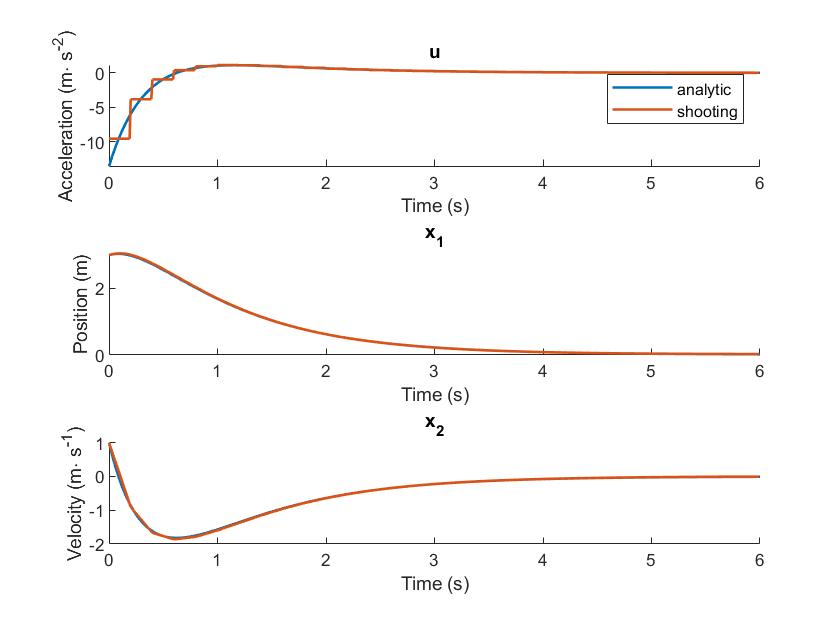
\includegraphics[width=0.8\textwidth]{Images/solution_zoh.jpg}
\caption{Direct optimization via a piecewise constant input.\\ Computation time: \SI{2.44}{\second}}
\label{fig:solution_zoh}
\end{figure}


\section{Multiple Shooting}

\par With multiple shooting, $u$ is parameterized in the same way as single shooting (see \ref{sec:singleshooting}). The main difference between multiple shooting and single shooting is that the ODE is calculated for each time interval separately. This ODE uses as initial value $s_i$ and is expressed as
\begin{equation}
    \dot{x}_i (t; s_i; q_i) = f(x_i(t;s_i,q_i),q_i), \qquad t\in [t_i; t_{i+1}]
    \label{eq:ode_multiple}
\end{equation}

\par Continuity of state $x$ for each time-step has to be assured. As a result, an equality constraint has to be added to the problem. This constraint is given by 
\begin{equation}
    \label{eq:shooting_constraint}
    s_{i+1} = x_i (t_{i+1}, s_i, q_i), \qquad i = 0,1,\dots, N-1
\end{equation}
where the path cost $l_i$ can now be calculated for each time interval $t \in [t_i; t_{i+1}]$ and is given by
\begin{equation}
    l_i(s_i;q_i) = \int_{t_i}^{t_{i+1}} L(x(t;s_i;q_i),q_i)dt 
\end{equation}

\par The optimization problem can now be redefined as
\begin{equation}
    \label{eq:cost_mul_shoot}
    \begin{aligned}
    & \underset{q,s}{\text{minimise}} && \sum_{i=0}^{N-1} l_i(s_i,q_i) + \psi (s_N) \\
    & \text{subject to}  && a(0) = x_0, \\
        & && s_{i+1} = x_i (t_{i+1}, s_i, q_i), &&& i = 0,1,\dots, N-1, \\
        & && h(s_i,q_i) \geq 0, &&& 1,\dots,N, \\
        & && r(x(T)) = 0
    \end{aligned}
\end{equation}

\par For a solution $u$ to be obtained with the same duration and order as in single shooting, the optimising algorithm will have to search through twice the amount of variables (an $s_i$ for every $q_i$). However, the larger search space will be sparse due to the presence of constraints, and, as a result, easier to solve, compared to the small and dense optimization problem produced by single shooting \cite{rao2009survey}.

\par Solutions for multiple shooting will be identical to single shooting and will differ only in computation time. As a result, examples with this method will not be given.

\section{Quadratic Programming}

\par Quadratic programming problems \cite{frank1956algorithm} have the form
\begin{equation}
    \label{eq:gen_quad_prog}
    \begin{aligned}
    & \underset{\overline{x}(.)}{\text{minimise}} && \frac{1}{2} \overline{x}^T H \overline{x} + f^T  \\
    & \text{subject to} && A \cdot \overline{x} \leq b, \\
    & && Aeq \cdot \overline{x} = beq, \\
    & && lb \leq \overline{x} \leq ub
    \end{aligned}
\end{equation} 
and are not specifically designed to tackle motion planning problems. The first step in applying quadratic programming to optimal control problems is to discretise the system's dynamics. 
\par A discrete linear system can be represented as
\begin{equation}
    \label{eq:discrete_state_space} 
    \phi_{x_k} + \Gamma_{u_k} - x_{k+1} = 0,
\end{equation}
where $x_k$ and $u_k$ are the state and input, respectively, at discrete time $k$, and $\Phi$ and $\Gamma$ are state and input matrices, respectively of appropriate dimensions.
\par The cost function to optimise that is equivalent to $\ref{eq:quadratic_cost}$ is given by
\begin{equation}
    J_d = x_N^T Q x_N + \sum_{k=0}^{N-1} x_k^T Q x_k + u_k^T R u_k
    \label{eq:discrete_quad_cost}
\end{equation}
where the matrices $Q$ and $R$ will be identical to the continuous time problem.

\par The goal of the quadratic programming optimiser is to obtain values $x_k$ and $u_k$ for all discrete-times that minimise \ref{eq:discrete_quad_cost}. In order to formulate the optimization problem in the form of \ref{eq:gen_quad_prog}, all of the variables to optimise have to be flattened to the column vector \begin{equation}
    \label{eq:quad_prog_xbar}
    \overline{x} = \begin{bmatrix} x^0_1\ \dots \ x^0_n & u_1^0\ \dots\ u_m^0 & (\dots) & x_1^{N-1}\ \dots\ x_n^{N-1} & u_1^{N-1}\ \dots\ u_m^{N-1} &  x_1^N\ \dots\ x_n^N \end{bmatrix} ^T,
\end{equation}
where the superscript is the iteration number that goes from 0 to $N$, $n$ is the dimension of $x$ and $m$ is the dimension of $u$. There will be a total of $(N-1)(n+m)+n$ variables to optimise.
\par To optimise \ref{eq:discrete_quad_cost}, matrix $H$ will be constructed by repetition of matrices $Q$ and $R$ as follows
\begin{equation}
    \label{eq:quad_prog_h}
    H = \begin{bmatrix}
        [Q] & & & & & \\
        & [R] & & & &  \\
        & & \ddots & & & \\
        & & & [Q] & & \\
        & & & & [R] & \\
        & & & & & [Q]
    \end{bmatrix}
\end{equation}

\par The system dynamics \ref{eq:discrete_state_space} will impose "dynamic" linear constraints given by
\begin{equation}
    \label{eq:quad_prog_Aeq_dyn}
    \underbrace{\begin{bmatrix}
        [\phi] & \left[\Gamma\right] & \left[ -I \right] & & \ldots \\
        & & [\Phi] & [\Gamma] & \left[ -I \right] & \ldots \\
        \vdots & \vdots & \vdots & \vdots & \vdots & \ddots 
    \end{bmatrix}}_\text{Aeq (dynamics)}
    \overline{x} = \underbrace{\begin{bmatrix} 0 \\ 0 \\ 0 \\ \vdots \\ 0 \end{bmatrix}}_\text{beq dynamics}
\end{equation}
where $I$ is the identity matrix with size equal to the dimension of $x$.

\par The first and last samples of $x$ will be restricted to the initial and final conditions, $x_i$ and $x_f$
\begin{equation}
    \label{eq:quad_prog_Aeq_init}
    \underbrace{\begin{bmatrix} 
        1 & 0 & 0 & \ldots & 0 \\
        0 & 1 & 0 & \ldots & 0 
    \end{bmatrix}}_\text{Aeq (initial state)}
    \overline{x} = \underbrace{\mathbf{x}^i}_\text{beq (initial state)}
\end{equation}
\begin{equation}
    \label{eq:quad_prog_Aeq_final}
    \underbrace{\begin{bmatrix} 
        0 & \ldots & 0 & 1 & 0 \\
        0 & \ldots & 0 & 0 & 1 
    \end{bmatrix}}_\text{Aeq (final state)}
    \overline{x} = \underbrace{\mathbf{x}^f}_\text{beq (final state)}
\end{equation}

\par The final matrices $Aeq$ and $beq$ that will be inserted into in the optimization software will be given by

\begin{equation}
    \label{eq:quad_prog_Aeq_total}
    \underbrace{\begin{bmatrix}
        \text{Aeq (dynamics)} \\ \text{Aeq (initial state)} \\ \text{Aeq (final state)}
        \end{bmatrix}}_\text{Aeq}
    \overline{x} =
    \underbrace{\begin{bmatrix}
        \vec{0} \\ x^i \\ x^f
        \end{bmatrix}}_\text{beq}
\end{equation}

\par An additional inequality constraint may be used to bound values of $\overline{x}$. These are coded in the $lb$ and $ub$ vectors which correspond to the lower bound and upper bounds for $\overline{x}$. Later, in the application examples, this will be used to bound the values of $u$.


\par In order to control the double integrator using quadratic programming techniques, the system's discrete-time equivalent will have to be obtained first. Matrices $\Phi$ and $\Gamma$ can be obtained via the Matlab function \texttt{c2d}. $H$ will be as described with $Q$ and $R$ identical to the analytical solutions; $f$ will be zero because there are no non-squared components of the cost function. Figure \ref{fig:solution_quad_prog_un} shows the solution of the quadratic problem for an unconstrained input and identical initial conditions to the analytical example were used.

%Within the context of motion control, these can be used to bound the input $u$, which, in this case, corresponds to leaving every corresponding variable of $\overline{x}$ to $U_{\text{max}}$ or $U_{\text{min}}$ and all others to $\pm \infty$ as shown in \ref{eq:quad_prog_ineq_constr}.
\par Figure \ref{fig:solution_quad_prog_con} shows the solution to a problem where $u$ is bounded by
\begin{equation}
\label{eq:quad_prog_ineq_constr}
\begin{gathered}
    ub = U_{\text{max}} \begin{bmatrix} \infty & \infty & 1 & \ldots & \infty & \infty & 1 & \infty & \infty \end{bmatrix} \\
    lb = U_{\text{min}} \begin{bmatrix} \infty & \infty & 1 & \ldots & \infty & \infty & 1 & \infty & \infty \end{bmatrix} 
\end{gathered}
\end{equation}
where $U_{\text{max}}$ and $U_{\text{min}}$ are given are given by $\pm 1$. Here we can see a clear saturation on the input up to time $\SI{2.5}{\second}$ after which the system evolves like in the unconstrained example.

\begin{figure}[h!]
\centering
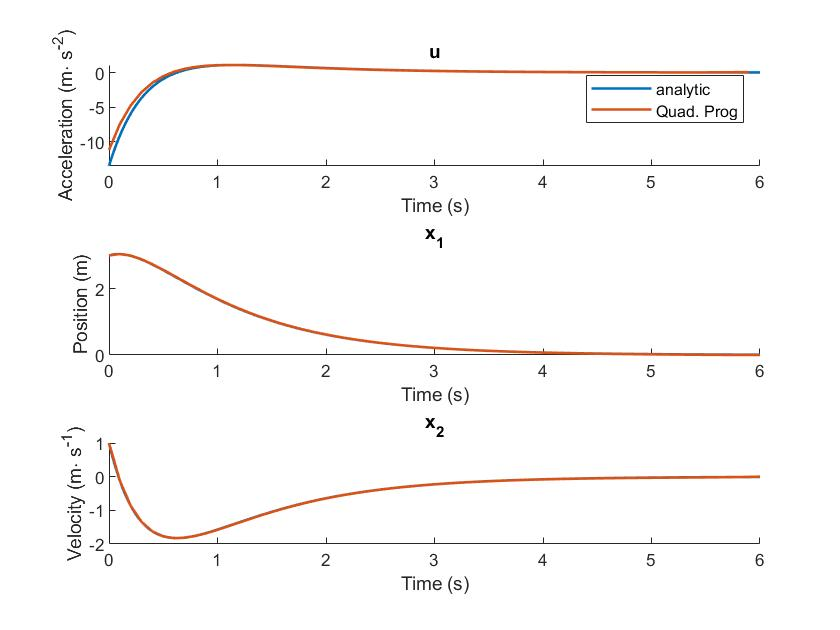
\includegraphics[width=0.75\textwidth]{Images/quad_prog_unconstrained.jpg}
\caption{Quadratic Programming solution}
\label{fig:solution_quad_prog_un}
\end{figure}


\begin{figure}[h!]
\centering
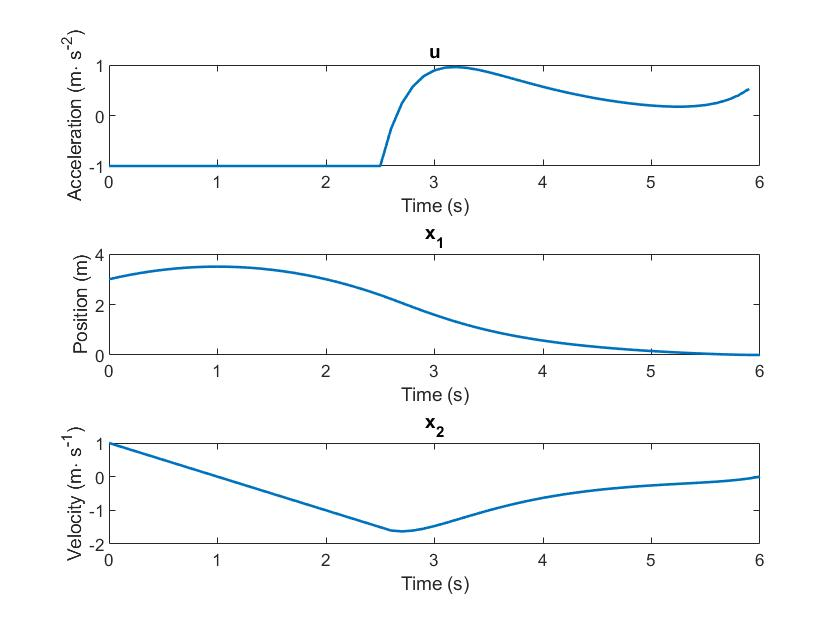
\includegraphics[width=0.75\textwidth]{Images/quad_prog_constrained.jpg}
\caption{Quadratic Programming solution with bounded input}
\label{fig:solution_quad_prog_con}
\end{figure}


\section{Monomial Polynomials}

\par Another way to describe trajectories is by using polynomials. If an optimal trajectory can be modelled by a polynomial, then it can be parameterized in terms of the polynomial's coefficients. As a result, the optimization problem tends to have a much smaller search space compared to, for example, shooting methods because with a relatively low order of polynomial, a whole trajectory over time $t\in [0,T]$ can be obtained will a relatively good cost. 
\par Polynomial methods are especially suited to deal with \textit{differentially flat systems} (see section \ref{sec:differentiallyflatsystems}). In differentially flat systems, the state and input variables can be directly expressed, without integrating any differential equation, in terms of the flat output and a finite number of its derivatives \cite{fliess1995flatness}. This means that with coefficients that describe just the flat output it is possible to describe all of the other variables of the system, thus resulting in a 

\par The solution provided by the Matlab function \texttt{fmincon} for the same double integrator problem of section \ref{sec:linearquadraticregulator} with this method will be a polynomial $\overline{p}$ for $x_1$. Once the optimal coefficients have been obtained the trajectories for $x_1$, $x_2$ and $u$ can be obtained by polynomial derivation and evaluation. This is possible because the system is differentially flat. These polynomials are related in the system of equations
\begin{equation}
    \label{eq:polys_of_double_integrator}
    \begin{cases}
        u (t) = a_0 + a_1 t + a_2 t^2 + \ (\dots) \\
        x_2 (t) = v_0 + a_0 t + \frac{a_1}{2} t^2 + \frac{a_2}{3} t^3 + \ (\dots)  \\
        x_1 (t) = p_0 + v_0 t + \frac{a_0}{2} t^2 + \frac{a_1}{6} t^3 + \frac{a_2}{12} t^4 + \ (\dots)
    \end{cases}
\end{equation}
 The cost function will be the same as the one used for the analytic method, and with the same initial conditions (see \ref{eq:my_cost} and \ref{eq:initial_conds}).
\par Figure \ref{fig:solution_pol} shows the solution of a polynomial optimization problem for a polynomial of order 7. Higher orders where attempted but take too long to converge. %Here, the variable to optimise $\overline{p}$ contains the coefficients that describes $x_1$. Because the system is deferentially flat, both $x_2$ and $u$ can be obtained as a function of $\overline{p}$  and will also be polynomials.


\par In order to guarantee the initial and final conditions of the state variable $x$, the linear constraint that has to be introduced is given by
\begin{equation}
    \label{eq:pol_equality}
    \underbrace{\begin{bmatrix}
    0 & 0 & \dots & 0 & 1 \\
    0 & 0 & \dots & 1 & 0 \\
    T^N & T^{N-1} & \dots & T & 0 
    \end{bmatrix}}_\text{Aeq} \overline{p}  =
    \underbrace{\begin{bmatrix} x_1^i \\ x_2^i        \\ 0 \end{bmatrix}}_\text{beq}
\end{equation}


\begin{figure}[h!]
\centering
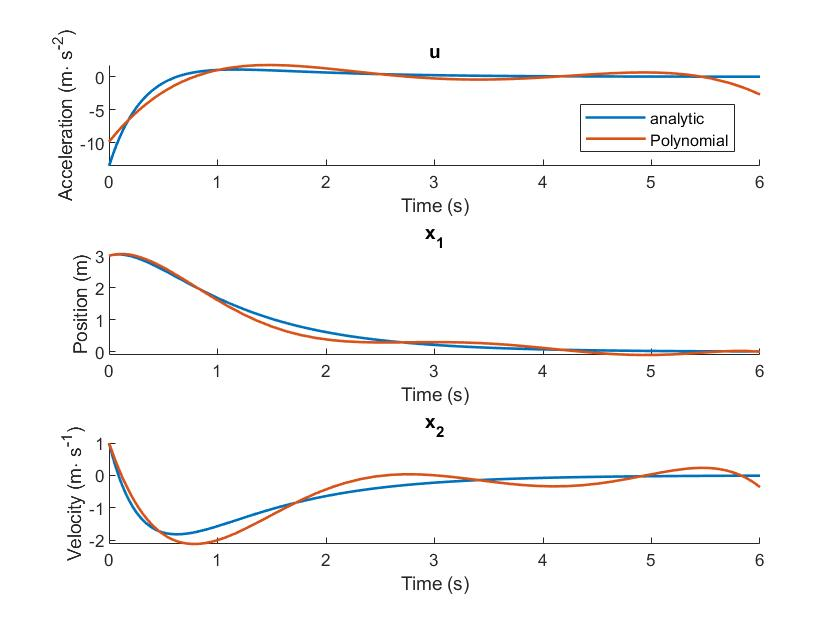
\includegraphics[width=0.8\textwidth]{Images/solution_pol.jpg}
\caption{Direct optimization with Polynomials. \\ Polynomial order: 7. \\
Computation time: \SI{1.33}{\second}}
\label{fig:solution_pol}
\end{figure}



\section{Bezier Curves}
\label{sec:bezcurves}
\par A Bezier curve is a parametric curve used in computer graphics and related fields. The curve, is named after Pierre Bezier, who used it in the 1960s for designing curves for the bodywork of Renault cars \cite{hazewinkelmichiel1997}.  Other uses include the design of computer fonts and animation \cite{hazewinkelmichiel1997}. 
The mathematical basis for Bezier curves, the Bernstein polynomials, was established in 1912, but the polynomials were not applied to graphics until some 50 years later when mathematician Paul de Casteljau in 1959 developed de Casteljau's algorithm, a numerically stable method for evaluating the curves, and became the first to apply them to computer-aided design at French auto-maker Citroen \cite{GeraldFarin2002}. 

\par What follows is a brief summary of the type of Bernstein polynomials that are exploited in this study.

\par A Bernstein polynomial is given by % represented as
\begin{equation}
    \label{eq:bern_pol}
    P(\tau) = \sum_{k=0}^n \overline{p}_k B_{k,n} (\tau), \qquad \tau\in [0,1]
\end{equation}
where $n$ is the order of the polynomial and $\tau$ is the time contraction of $t$, given by 
\begin{equation}
    \tau = \frac{t}{T}, \qquad t\in [0,T].
    \label{eq:time_delay}
\end{equation}
\par The $p_k$ are the polynomial coefficients or \textit{control points}, and $b_k^n$ are the \textit{Bernstein Basis}, given by 
\begin{equation}
	B^n_k {(\tau)} = \binom{n}{k} {(1 - \tau)}^{n-k} \tau^k
    \label{eq:bern_basis}
\end{equation}
As a result, a Bernstein polynomial of order $n$ is a linear combination of $(n+1)$ Bernstein basis with weights given by $p_k$. The Bernstein Basis, as a function of $\tau$, for 6 different orders, $n$, are shown in figure \ref{fig:bernsteinbasis}.

\begin{figure}[h!]
\centering
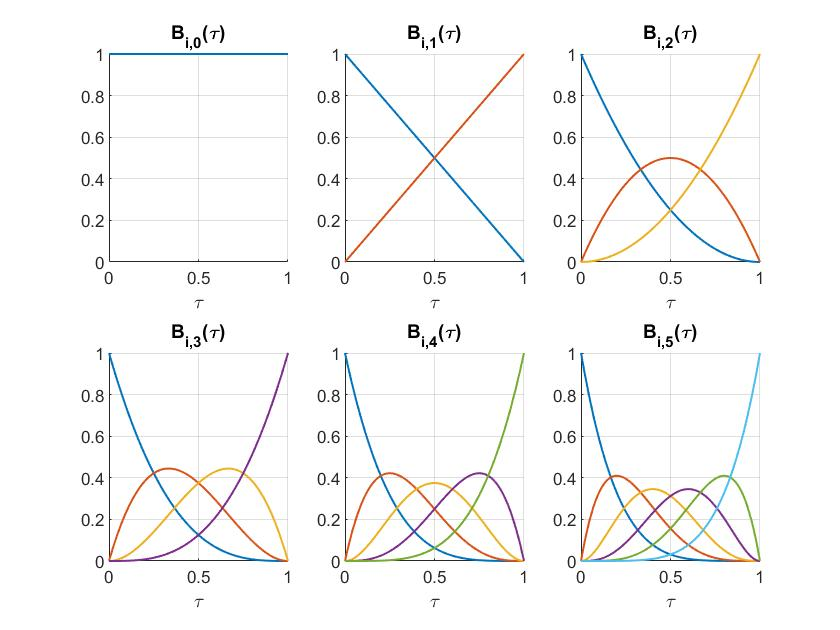
\includegraphics[width=0.8\textwidth]{Images/bernstein_basis.jpg}
\caption{Representation of the Bernstein Basis for $\tau \in [0,1]$ for orders $n=0\cdots 5$}
\label{fig:bernsteinbasis}
\end{figure}

\par For a polynomial of order $n$, the $i \in {0 .. n}$ control points can be represented as a vector on a vector $p$. For example, if $p$ is given by 
\begin{equation}
    \overline{p} = \begin{bmatrix}0\\ 0.5\\ 1\\ 0.7\\ 0.3\\ -0.7\\ -1\\ -0.5\\ -0.1\end{bmatrix},
\end{equation}
the plot of the polynomial given by these coefficients is shown in figure \ref{fig:generic_bezier}. The control points on vector $p$ are plotted along time in equidistant time nodes. What can be seen is that the control points "attract" the curve towards themselves.

\begin{figure}[h!]
\centering
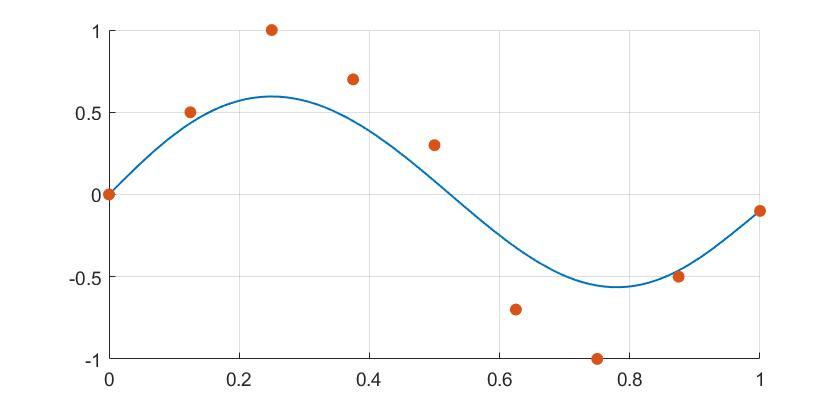
\includegraphics[width=0.8\textwidth]{Images/generic_bezier.jpg}
\caption{A Bernstein Polynomial}
\label{fig:generic_bezier}
\end{figure}


\par Two or three Bernstein polynomials of the same order, i.e., same number of control points, can be plotted against each other within the time domain $\tau \in [0,1]$. The control points of the curves together form $n+1$ points in two or three dimensions. These two or three dimension polynomials are also known as Bezier curves. Figure \ref{fig:generic_bezier} shows a 2-D Bezier Curve, the control points which resulted in it are plotted too. The control points for this curve had a specific order on the underlying Bernstein Polynomial. Changing the oder of the control points on the polynomial will, as a result, produce a different Bezier curve, such as the one in figure \ref{fig:generic_bezier2D_reordered}, despite the control points being the same on the 2-D plot.

\begin{figure}[h!]
\centering
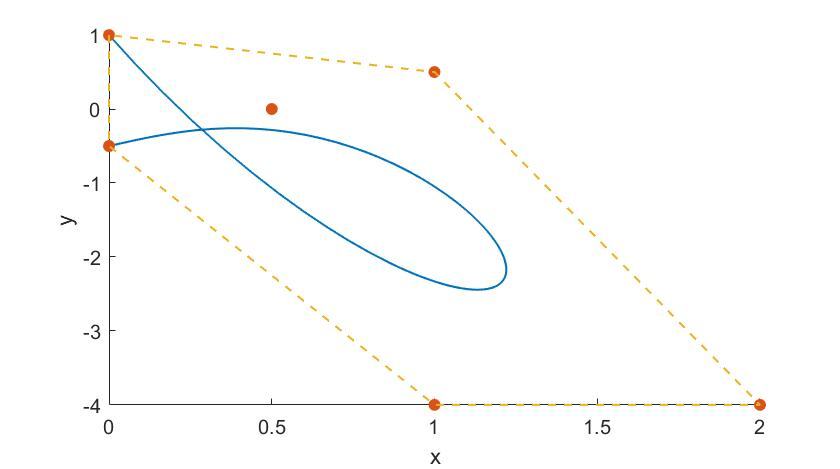
\includegraphics[width=0.8\textwidth]{Images/generic_bezier2D.jpg}
\caption{A 2-D Bernstein Polynomial}
\label{fig:generic_bezier2D}
\end{figure}

\begin{figure}[h!]
\centering
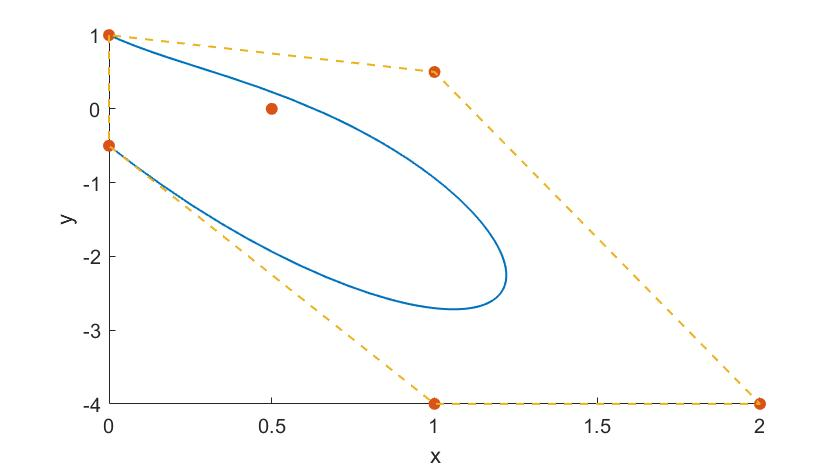
\includegraphics[width=0.8\textwidth]{Images/generic_bezier2D_reordered.jpg}
\caption{A 2-D Bernstein Polynomial with Reordered Control Points}
\label{fig:generic_bezier2D_reordered}
\end{figure}


\par One property than can be observed in figure~\ref{fig:generic_bezier} is that, within the domain $t \in [0,T]$, the polynomial is limited by a convex hull \cite{cichella2018bernstein} formed by the control points.
\par The initial and final values of $P(t)$ in the interval $[0,T]$ are given by
\begin{equation}
    \label{eq:bern_in_fin}
    \begin{gathered}
        P(0) = p_{n,0} \\
        P(T) = p_{n,n}
    \end{gathered}
\end{equation}
and the derivative and integral are given by 
\begin{equation}
    \label{eq:bern_deriv}
    \dot{P}(t) = \frac{n}{T} \sum_{k=0}^{n-1} (p_{k+1,n} - p_{k,n}) B_{k,n-1}(t)
\end{equation}
\begin{equation}
    \label{eq:bern_int}
    \int_0^T P(t)dt = \frac{T}{n+1} \sum_{k=0}^{n} p_{k,n}
\end{equation}

\par The control points for the derivative of a bernstein polynomial can be obtained my a multiplication of a derivation matrix by the control points of the original curve stored in the column vector, with the matrix given by 
\begin{equation}
    \boldsymbol{D}_{N-1} = 
    \begin{bmatrix}
        -\frac{N}{T} & \frac{N}{T} & 0 & \ldots & & 0 \\
        0 & -\frac{N}{T} & \frac{N}{T} & \ldots & & 0 \\
        \vdots &  \ddots & \ddots & \ddots & &   \\
        0 & & \ldots & & -\frac{N}{T} & \frac{N}{T}
    \end{bmatrix} \in \mathbb{R}^{(N+1)\times N}
    \label{eq:bernderivmat}
\end{equation}

\par The control points of the Anti-Derivative/Primitive can be obtained similarly to the derivation by multiplying the control points to a primitive matrix \cite{privateconversationprimitive}, and adding a vector:
\begin{equation}
    p = A \cdot \dot{p}  + p_0
\end{equation}
where $p_0$ is the initial values of $P$ and the matrix A is given by 
\begin{equation}
    \boldsymbol{A}_{N+1} = \begin{bmatrix}
        0 & 0 & \ldots & 0 & 0 \\
        \frac{T}{N+1} & 0 & \ldots & 0 & 0 \\
        \frac{T}{N+1} & \frac{T}{N+1} & \ldots & 0 & 0 \\
        \vdots & \ddots & \ddots & \ddots & \\
        \frac{T}{N+1} & \frac{T}{N+1} & \ldots & \frac{T}{N+1} & \frac{T}{N+1} \\
    \end{bmatrix}
\end{equation}

\par A Bernstein polynomial of degree $N$ and coefficients $p_{k,N}\in \mathbb{R}, k = 0,\dots,N$ can be expressed as a Bernstein polynomial of degree $M$ with $M>N$, with coefficients $p_{k,M} \in \mathbb{R}, k = 0,\dots,M$ given by 
\begin{equation}
    p_{k,M} = \sum_{j=\text{max}(0,k+M-N)}^{\text{min}(N,k)} \frac{{M-N \choose k-j}{N\choose j}}{{M\choose k}} p_{j,N} \in \mathbb{R}^n,
\end{equation}
which is known as degree elevation. In other words, it is possible find a polynomial with $M+1$ control points such that it's identical to a curve with order $N+1$ within time $t\in[0,T]$.
\par The control points for the degree elevation can also be obtained by multiplying the control points vector by a matrix $\boldsymbol{E}$ whose indices are given by 
\begin{equation}
    \label{eq:bernsteinelevindices}
    \boldsymbol{E}_{ij} = \frac{{N\choose j}{M-N\choose i-j}}{{M\choose i}}
\end{equation}


%\par The cost function, which will be the same as previous the previous examples, (\ref{eq:my_cost}). In order to calculate it and take, equations \ref{eq:bern_mul} and \ref{eq:bern_sum} will be necessesary for summation and addition of Bernstein polynomials, respectfully.
\par Multiplication and addition is given by
\begin{equation}
    \label{eq:bern_mul}
    f(t)g(t) = \sum^{m+n}_{i=0}  \left(\sum_{i=\text{max}(0,i-n)}^{\text{min}(m,i)} \frac{\binom{m}{j}\binom{n}{i-j}}{\binom{m+n}{i}} f_{j,m}g_{i-j,n}\right) B_{i,m+n}(t)
\end{equation}
\begin{equation}
    \label{eq:bern_sum}
    f(t)\pm g(t) = 
    \sum^{m}_{i=0}  \left(f_{i,n} \pm \sum_{j=\text{max}(0,i-m+n)}^{\text{min}(n,i)} \frac{\binom{n}{j}\binom{m-n}{i-j}}{\binom{m}{i}} g_{j,n}\right) B_{i,m+n}(t)
\end{equation}

\par The De Casteljau's algorithm \cite{shene2012finding} is a recursive method to evaluate polynomials in Bernstein form. A geometric interpretation of this algorithm presented as follows:
\begin{enumerate}
    \item Connect the consecutive control points in order to create the control polygon of the curve;
	\item Subdivide each line segment of this polygon with the ratio $t:(1-t)$ and connect the obtained points which results in a new polygon with one fewer control points;
    \item Repeat the process until a single point is achieved – this is the point of the curve corresponding to the parameter $t$.
\end{enumerate}

Figure~\ref{fig:deCasteljau} illustrates the breakdown of the control points into polygons and sub polygons. 
\par The evaluation of the curve can be carried out analytically. For a Bernstein Polynomial $\boldsymbol{x}_N:[0,t_f]\rightarrow \mathbb{R}^n$, and a scaler $t_{div}\in [0,t_f]$, the Bernstein polynomial at $t_{div}$ can be computed using the following recursive relation:
\begin{equation}
\begin{gathered}
    \overline{\boldsymbol{x}}^{[0]}_{i,N} = \overline{\boldsymbol{x}}_{i,N},\quad i=0,\dots, N  \\
    \overline{\boldsymbol{x}}^{[j]}_{i,N} = \overline{\boldsymbol{x}}^{[j-1]}_{i,N} \frac{t_f-t_{div}}{t_f} + \overline{\boldsymbol{x}}^{[j-1]}_{i+1,N} \frac{t_{div}}{t_f}
\end{gathered}
\end{equation}
with $i=0,\dots, N-j$, and $j=1,\dots, N$. Then, the Bernstein polynomial evaluated at $t_{div}$ is given by
\begin{equation}
    \overline{\boldsymbol{x}}_N(t_{div}) = \overline{\boldsymbol{x}}_{0,N}^{[N]}.
\end{equation}
Moreover, the Bernstein polynomial can be subdivided at $t_{div}$ into two $N$th order Bernstein polynomial with Bernstein coefficients
\begin{equation}
    \overline{\boldsymbol{x}}^{[0]}_{0,N}, \overline{\boldsymbol{x}}^{[1]}_{0,N}, \dots, \overline{\boldsymbol{x}}^{[N]}_{0,N}, \quad \text{and}\quad \overline{\boldsymbol{x}}^{[N]}_{0,N}, \overline{\boldsymbol{x}}^{[N-1]}_{0,N}, \dots, \overline{\boldsymbol{x}}^{[0]}_{0,N}.
\end{equation}

\begin{figure}[h!]
\centering
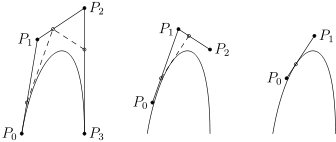
\includegraphics[width=0.8\textwidth]{Images/deCasteljau.png}
\caption{Visual representation of the De Casteljau algorithm}
\label{fig:deCasteljau}
\end{figure}

%\par A numerically stable method to evaluate Bernstein polynomials exists and is known as the \textit{deCasteljau} algorithm;

%\begin{description}
%    \item[$L$] is the lagrangian
%    \item[$\Psi$] is the terminal cost
%    \item[$f(x,t)$] is the dynamic model   
%\end{description}

The convex hull property of these polynomials will prove useful in an algorithm that calculates distance between curves, which will be used in deconfliction of trajectories in multiple vehicle control. By just knowing the position of the control points in the space, it is possible to guarantee constraint satisfaction in the whole trajectory and not just in the control points.

\par Just as with monomial polynomials, when these Bernstein polynomials are applied to differentially flat systems, a reduction of the number of parameters to optimise is possible because with just a flat output, all state variables can be derived. If the system is not differentially flat, then parameters for all state variables need to be defined and optimised but will be subject to the constrained imposed by the system's dynamics.
%The optimization problems developed for motion planning in this study center around the use of what is known as Bernstein polynomials.

\par The solution obtained by the Matlab function \texttt{fmincon} for the same double integrator problem of section \ref{sec:linearquadraticregulator} with this Bernstein polynomial based approach will provide the coefficients $\overline{p}$ for the Bernstein polynomial of state variable $x_1$. 

\par Figure \ref{fig:bernstein_1d} shows the solution for the same quadratic optimization problem and with the same initial conditions as the previous sections. The red circles in the figure show the distribution of the obtained coefficients. The resulting polynomial has order 14.

\par In order to guarantee that the initial and final conditions are respected, the linear constraint that has to be introduced is given by
\begin{equation}
    \label{eq:bern_equality}
    \underbrace{\begin{bmatrix}
        1 & 0 & 0 & \dots & 0 \\
        \frac{n}{T} & -\frac{n}{T} & 0 & \dots & 0 \\
        0 & 0 & 0 & \dots & 1 \end{bmatrix}}_{\text{Aeq}_{\text{1D}}} \overline{p} =
    \underbrace{\begin{bmatrix}
        x_0^i \\ x_1^i \\ 0\end{bmatrix}}_{\text{beq}_{\text{1D}}}
\end{equation}


\begin{figure}[h!]
\centering
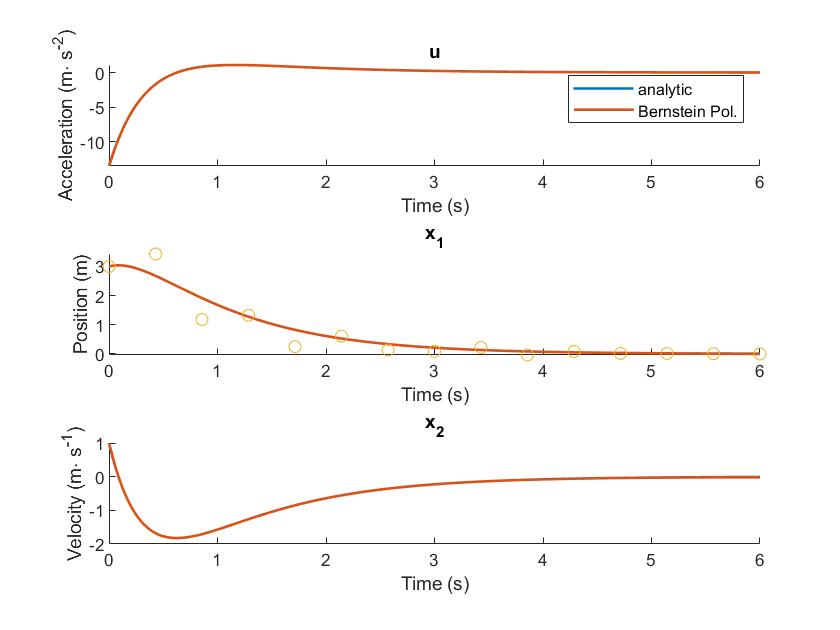
\includegraphics[width=0.8\textwidth]{Images/bernstein_1d.jpg}
\caption{Direct Bernstein Solution}
\label{fig:bernstein_1d}
\end{figure}

\section{Differentially Flat Systems}
\label{sec:differentiallyflatsystems}

\par A nonlinear system of the form
\begin{equation}
    \dot{x} = f(x(t),u(t)), \quad x(t) \in \mathbb{R}^n
\end{equation}
is said to be \textit{differentially flat} \cite{fliess1995flatness} or simply \textit{flat} if there exists a set of variables $y = (y_1, \dots, y_m)$ called the \textit{flat output}, such that
\begin{itemize}
    \item the components of $y$ are not differentially related over $\mathbb{R}$;
    \item every system variable, state or input, may be expressed as a function of the components of $y$ and a finite number of their time-derivatives, and 
    \item every component of $y$ may be expressed as a function of the system variables and of a finite number of their time-derivatives. 
\end{itemize}

\par The flat output has, in general, a clear physical interpretation and captures the fundamental properties of a given system and its determination allows to simplify considerably the control design. This implies that there is a fictitious \textit{flat output} that can explicitly express all states and inputs in terms of the flat output and a finite number of derivatives, thus reducing the number of parameters to be optimised.



\section{Remarks}

\par Out of all of the presented Direct Methods, the preferred is the Bernstein polynomials method because it provides fast solutions for the simple double integrator problem and, as will be seen in later chapters, will prove advantageous for differentially and non-differentially flat dynamic systems.
